
\chapter{Hardware and Software}

In the classical Von Neumann architecture there is only one processing unit (CPU) that processes instructions, the ALU is responsible for math and logic operations and the register stores data.

\begin{figure}[H]
    \centering
    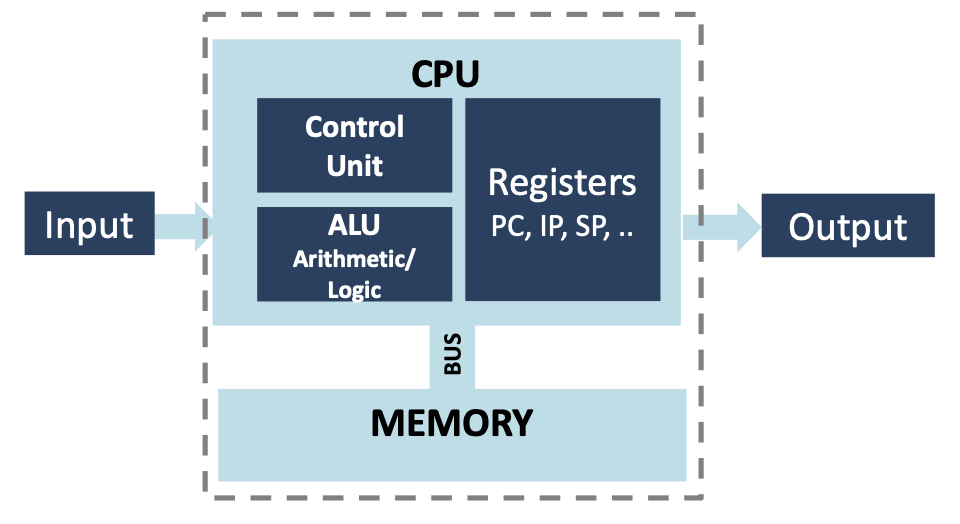
\includegraphics[width=0.8\textwidth]{assets/fig2.png}
    \caption{Von Neumann architecture}
    \label{fig:von_neumann_architecture}
\end{figure}

One instruction is executed at a time, the CPU fetches the instruction from the memory, decodes it and executes it. The CPU can access the memory to read or write data. Accessing any location in the mempory has always the same cost, this is called the \textbf{uniform memory access} (UMA).

\section{Moore's Law}

\begin{definitionblock}[Moore's Law]
    It states that the number of transistors in a dense integrated circuit doubles about every two years.
\end{definitionblock}

How can we go from Moore's Law to processor performance? Through Dennard Scaling:
\begin{quotation}
    "Power density stays constant as transistors get smaller"
\end{quotation}

Intuitively, 
\begin{itemize}
    \item \textbf{Smaller transistors} $\to$ shorter propagation delay $\to$ faster frequency
    \item \textbf{Smaller transistors} $\to$ smaller capacitance $\to$ lower voltage
\end{itemize}

\[
    Power \propto Capacitance \times Voltage^2 \times Frequency
\]

\textbf{But$\dots$} even with smaller transistors, we cannot continue reducting power, there are then two options: 
\begin{itemize}
    \item \textbf{Increase power}
    \item \textbf{Stop frequency scaling}
\end{itemize}

From 2006, single-core performance stopped increasing, so the only way to increase performance is to use more cores. The first solution is to write efficient software to make the efficient use of hardware resources. The second is to use specialized architectural solutions, like GPUs, FPGAs, etc.

Today, \textbf{CPUs are multicore processors}, lowering clock frequency because of power and heat dissipation, but packing more computing cores onto a chip. These cores will share some resources (memory, network, disk, $\dots$) but are still capable of independent calculations.

\begin{figure}
    \centering
    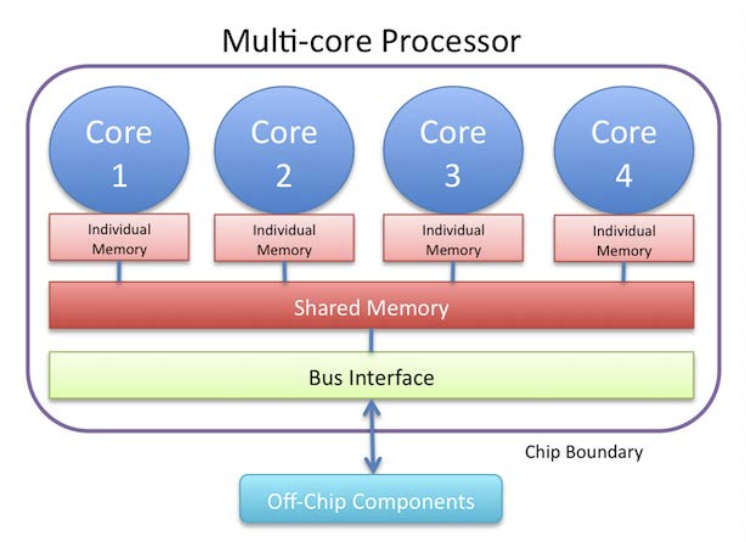
\includegraphics[width=0.8\textwidth]{assets/fig3.png}
    \caption{Multicore processors}
    \label{fig:multicore_processors}
\end{figure}

\section{Parallel Computers}

Flynn Taxonomy (1966) is used to classify parallel computers based on the number of instruction streams and data streams.

\begin{figure}[H]
    \centering
    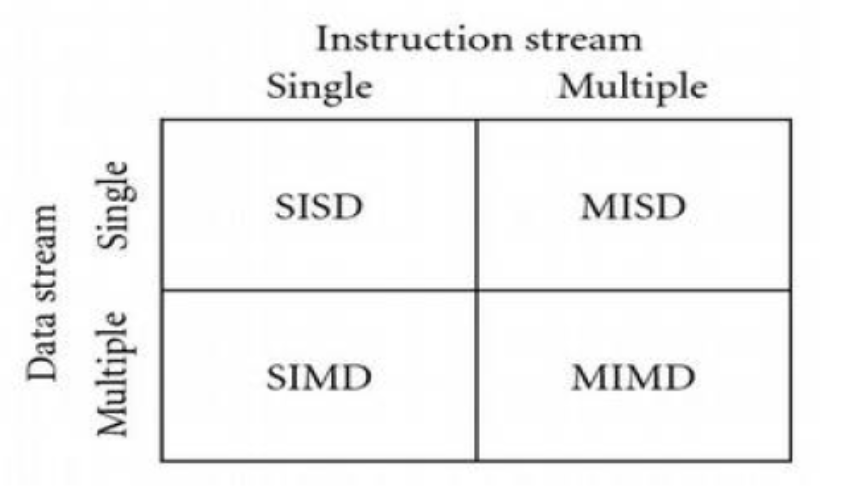
\includegraphics[width=0.6\textwidth]{assets/fig4.png}
    \caption{Flynn Taxonomy}
    \label{fig:flynn_taxonomy}
\end{figure}

\begin{figure}[H]
    \centering
    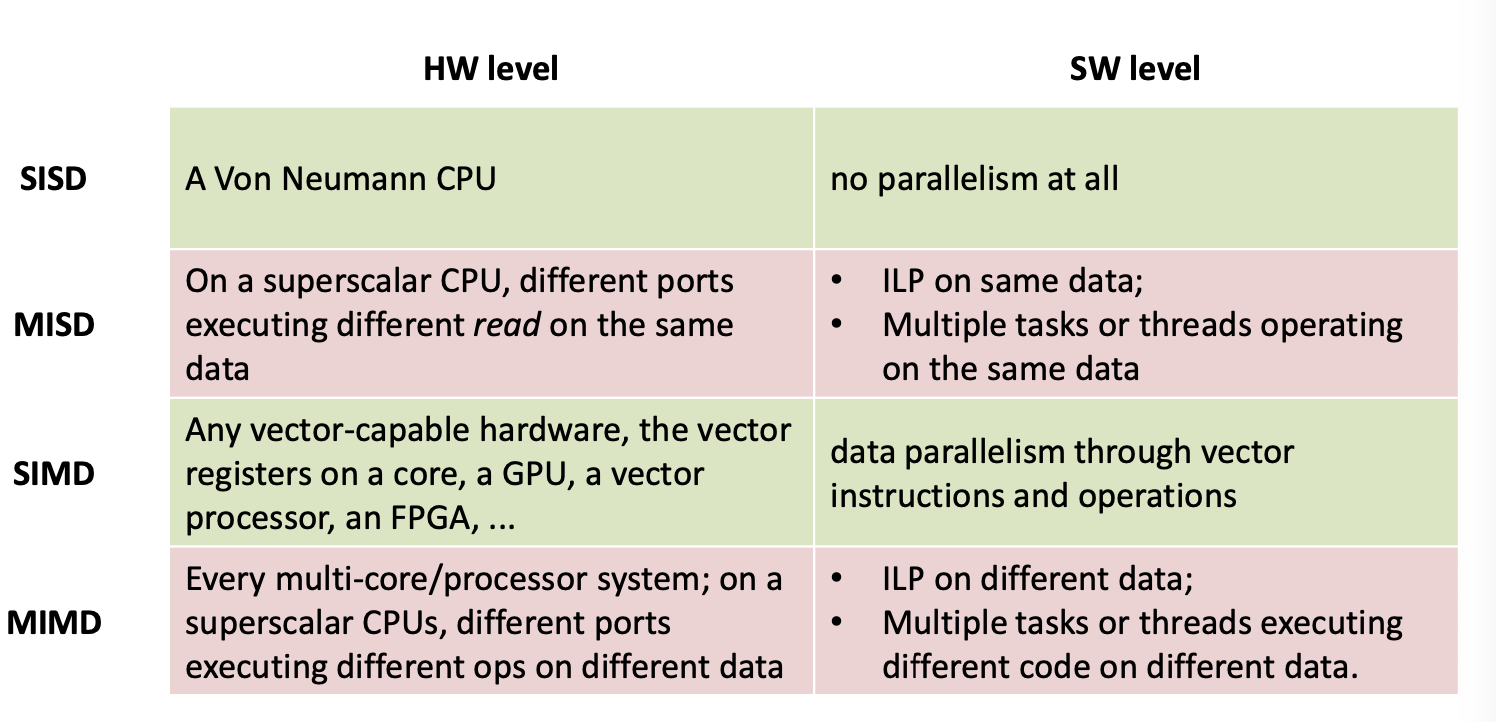
\includegraphics[width=0.8\textwidth]{assets/fig5.png}
    \caption{Parallel computers}
    \label{fig:parallel_computers}
\end{figure}

The essential components of a HPC cluster are:
\begin{itemize}
    \item \textbf{Compute nodes}: the actual computers that perform the calculations
    \item \textbf{Interconnect}: the network that connects the compute nodes
    \item \textbf{Storage}: the disk space where data is stored
    \item \textbf{Software}: the operating system and the software stack that runs on the cluster
\end{itemize}

\begin{figure}[H]
    \centering
    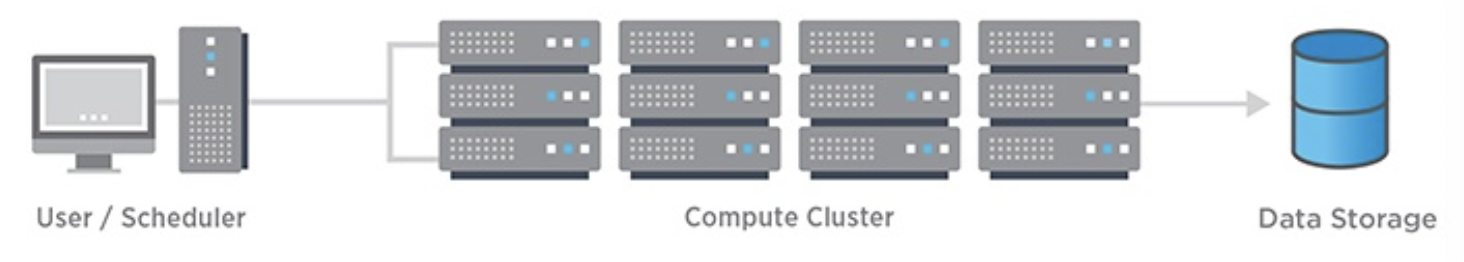
\includegraphics[width=0.8\textwidth]{assets/fig6.png}
    \caption{HPC cluster}
    \label{fig:hpc_cluster}
\end{figure}

\begin{minipage}{0.45\textwidth}
    A core is the smallest unit of computing, having one or more threads and is responsible for executing instructions. 
    \begin{figure}[H]
        \centering
        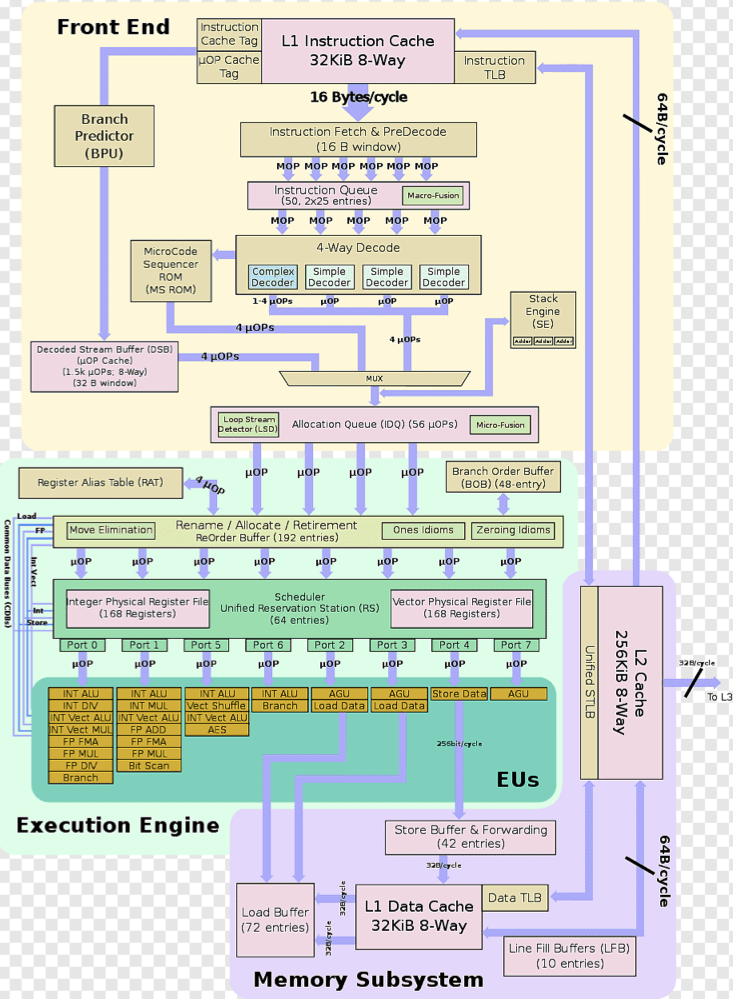
\includegraphics[width=0.5\textwidth]{assets/fig7.png}
        \caption{Core}
        \label{fig:core}
    \end{figure}
\end{minipage}
\begin{minipage}{0.45\textwidth}
    \begin{figure}[H]
        \centering
        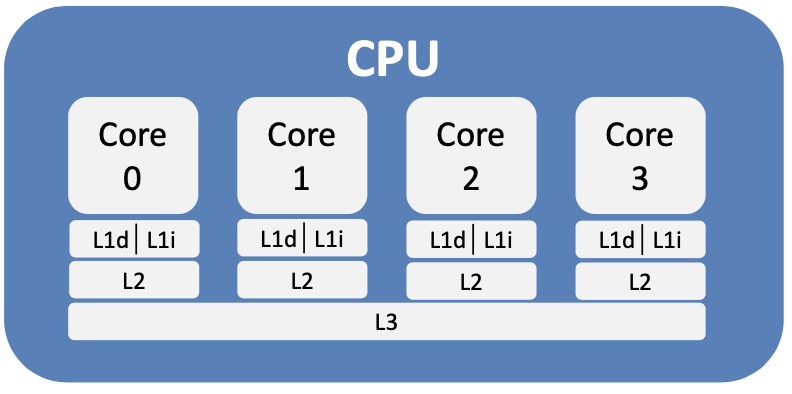
\includegraphics[width=0.5\textwidth]{assets/fig8.png}
        \caption{Cache hierarchy}
        \label{fig:cache_hierarchy}
    \end{figure}
    Cache hierarchy can have different topologies.
\end{minipage}

\begin{figure}[H]
    \centering
    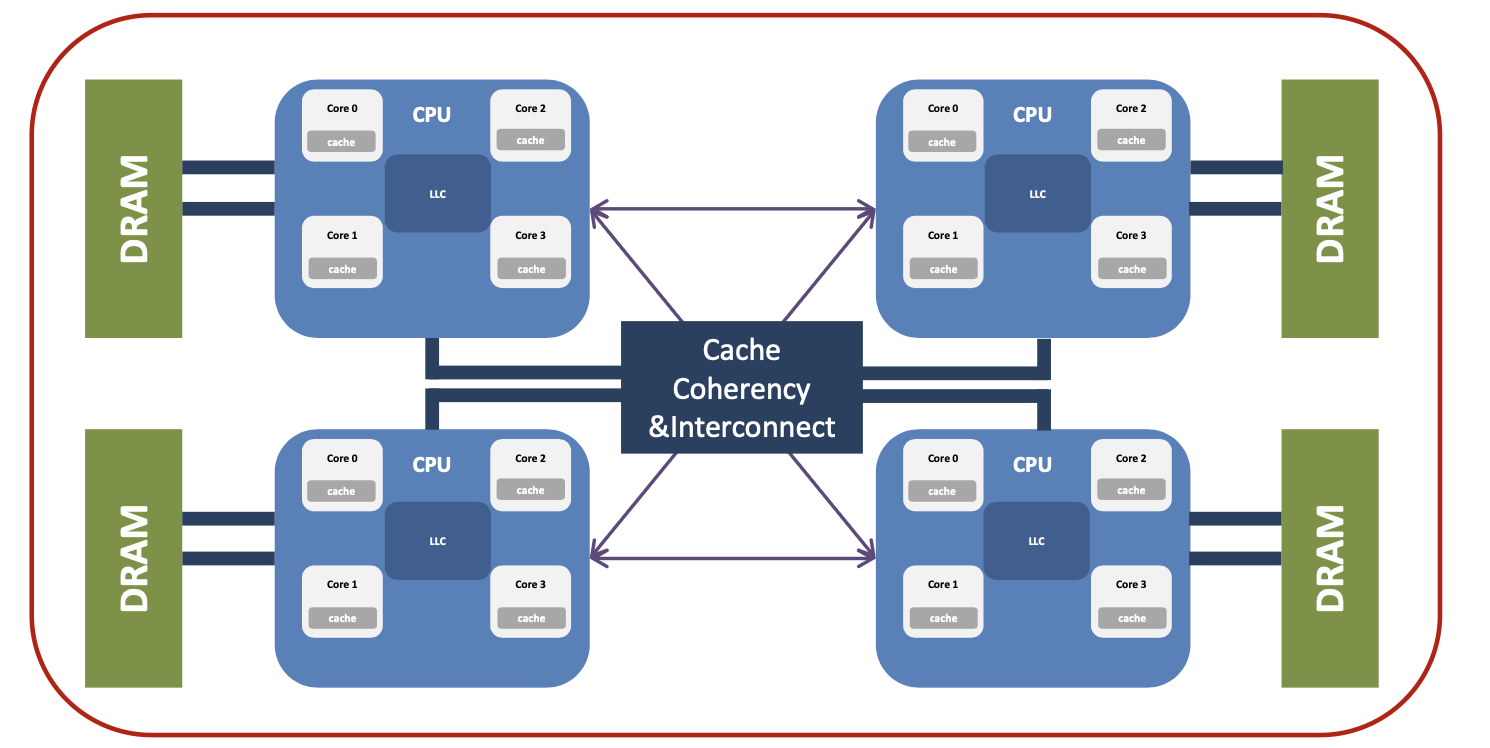
\includegraphics[width=0.8\textwidth]{assets/fig9.png}
    \caption{Node topology}
    \label{fig:node_topology}
\end{figure}

\begin{tipsblock}
    \textbf{Cache hierarchy} has been invented cause accessing memory (moving data) takes almost 100x times computing (doing operations). The cache is a small memory that stores the most frequently accessed data. The cache is faster than the main memory but smaller. The cache is divided into levels, the first level is the fastest but the smallest, the second level is slower but bigger, and so on.
\end{tipsblock}

In a cluster there are different types of networks:
\begin{itemize}
    \item \textbf{High-speed network}: used for communication between nodes (parallel computation, low latency/high bandwidth, infiniband or ethernet as examples)
    \item \textbf{I/O NETWORK}: used for communication with storage (I/O requests, latency not fundamental/good bandwidth, NFS, Lustre, GPFS as examples)
    \item \textbf{In band Management Network}: used for cluster management, monitoring, and control, LRMS (Load Resource Management System) as examples
    \item \textbf{Out of band Management Network}: used for cluster management, remote control of nodes and any other device, IPMI (Intelligent Platform Management Interface) as examples
\end{itemize}

What about \textbf{memory}?

It is fundamental and on a supercomputer there is a hybrid approach as for the memory placement. 
The memory on a single node can be accessed directly by all the cores on that node (\textbf{shared-memory}). 
When many nodes are used at a time, a process cannot directly access the memory on a different node, it needs to issue a request for that. That is named \textbf{distributed-memory}.

\subsection*{Shared Memory}
\begin{itemize}
    \item \textbf{Uniform Memory Access (UMA)}: 

    Each processor has uniform access to memory. Also known as symmetric multiprocessors (SMP).
    \begin{figure}[H]
        \centering
        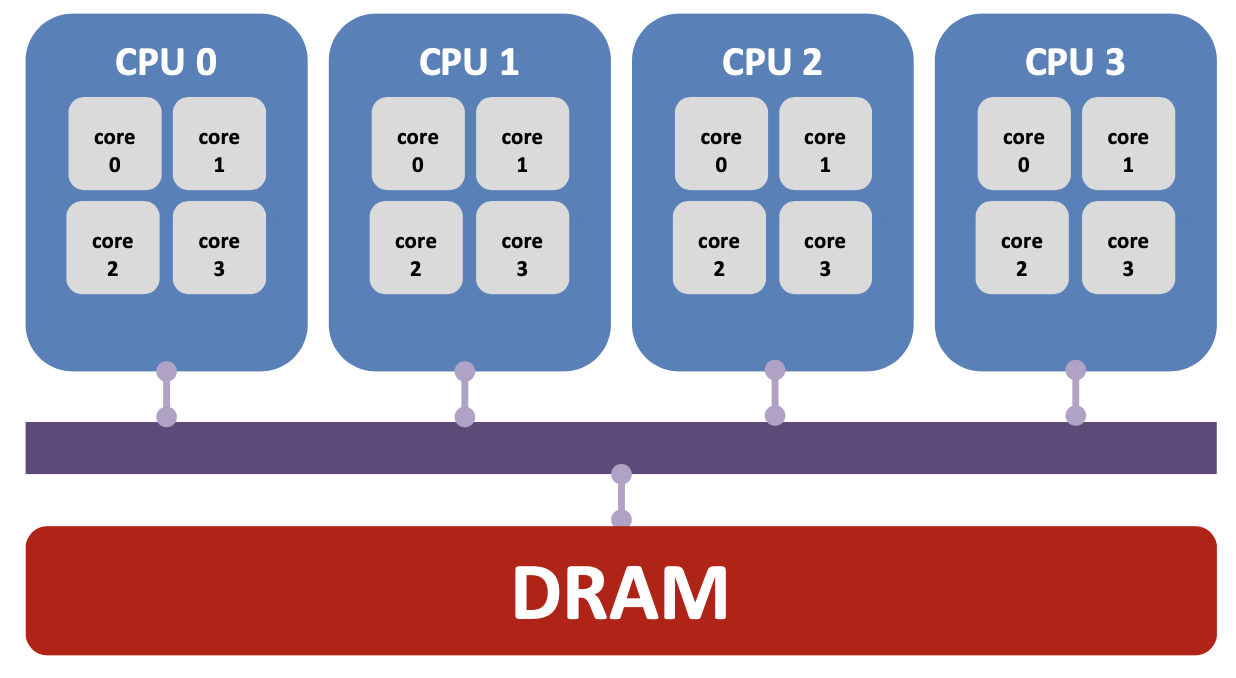
\includegraphics[width=0.6\textwidth]{assets/fig10.png}
        \caption{Shared memory - UMA}
        \label{fig:shared_memory}
    \end{figure}

    \item \textbf{Non-Uniform Memory Access (NUMA)}: Time for memory access depends on location of data. Local access is faster on non-local access. 
\end{itemize}

\begin{warningblock}[Challenges for multicore]
    It aggravates the \textbf{Memory Wall problem}, where the memory access time is much slower than the CPU speed.
    \begin{itemize}
        \item \textbf{Memory bandwidth}: the memory bandwidth is limited and shared among all the cores
        \item \textbf{Memory latency}: the memory latency is high and can be a bottleneck
        \item \textbf{Memory contention}: the memory contention can be a problem when multiple cores access the same memory location
    \end{itemize}
\end{warningblock}

\begin{minipage}{0.65\textwidth}
    \begin{figure}[H]
        \centering
        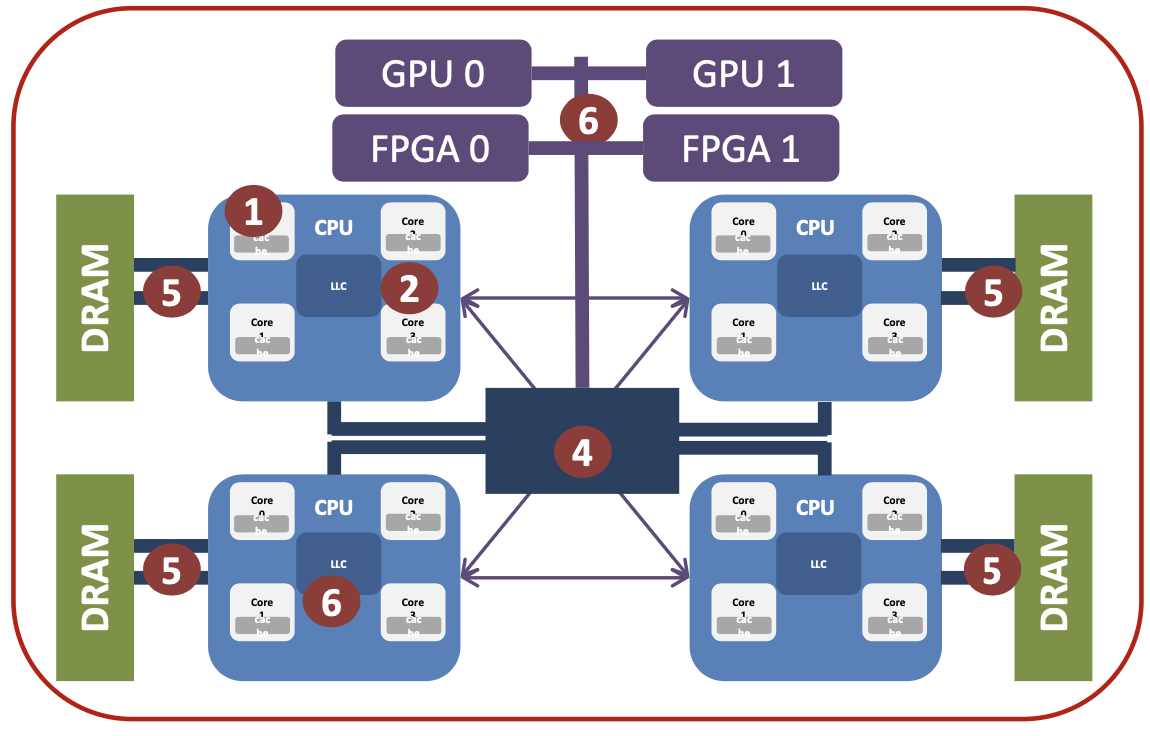
\includegraphics[width=0.9\textwidth]{assets/fig11.png}
        \caption{Parallelism within a HPC node}
        \label{fig:parallelism_hpc}
    \end{figure}
\end{minipage}
\begin{minipage}{0.25\textwidth}
    \begin{enumerate}
        \item ILP/SIMD units 
        \item Cores 
        \item 
        \item Socket/ccNuma domains 
        \item Inner cache levels 
        \item Multiple accelerators
    \end{enumerate}
\end{minipage}



